\documentclass[a4paper,12pt]{article} % тип документа
\usepackage[margin=1in]{geometry} % Поля

%  Русский язык
\usepackage[warn]{mathtext}
\usepackage[T2A]{fontenc}			% кодировка
\usepackage[utf8]{inputenc}			% кодировка исходного текста
\usepackage[english,russian]{babel}	% локализация и переносы
% Математика
\usepackage{amsmath,amsfonts,amssymb,amsthm,mathtools} 
\usepackage{wasysym}
%%%
\usepackage{graphicx}

\usepackage{tabularx}

\usepackage{gensymb} % знак градуса
\usepackage{enumitem} % изменить список enumerate
\usepackage{placeins} % \FloatBarrier

\renewcommand{\thesection}{\Roman{section}} 
\renewcommand{\thesubsection}{\roman{subsection}}


\begin{document}

\newcolumntype{Y}{>{\centering\arraybackslash}X} %new tabularx


%титул
\hrule 	
\medskip
\begin{raggedright}
{\large \textbf{Отчёт по работе 5.2.2 и 5.2.3}}
\\
\medskip
{\Large Изучение спектров атома водорода и молекулы йода} 
\\
\medskip
{\large Карташов Констанин, Бичина Марина Б04-005}
\medskip
\hrule
\medskip
\end{raggedright}


\section{Анотация}

\paragraph{Цель работы:} 
Изучить спектр излучение водорода. Изучить спектр поглощения паров йода.

\paragraph{Оборудование:}
\begin{itemize}
\renewcommand{\labelitemi}{$\triangleright$}
\itemsep0em
\item Монохроматор-спектрометр
\item Неоновая и Ртутная лампа для калибровки
\item Водородная лампа
\item Кювета с парами йода и лампа накаливания
\end{itemize}


\medskip\hrule\medskip

\section{Теоретическая часть}

\subsection{Спектр водорода}

\paragraph{} Длины волн спектральных линий водородоподобных атомов описываются формулой Бальмера:
\[
\frac{1}{\lambda_{n,m}} = RZ^2 \left( \frac{1}{n^2} - \frac{1}{m^2} \right),
\]
\noindent которая для серии Бальмера водорода ($n = 2, \; m \in \{3, 4, 5, 6 \}$) принимает вид:
\begin{equation}
\frac{1}{\lambda} = R \left( \frac{1}{4} - \frac{1}{m^2} \right)
\label{e:balmer}
\end{equation}

\subsection{Спектр йода}

\begin{figure}[h]
\centering
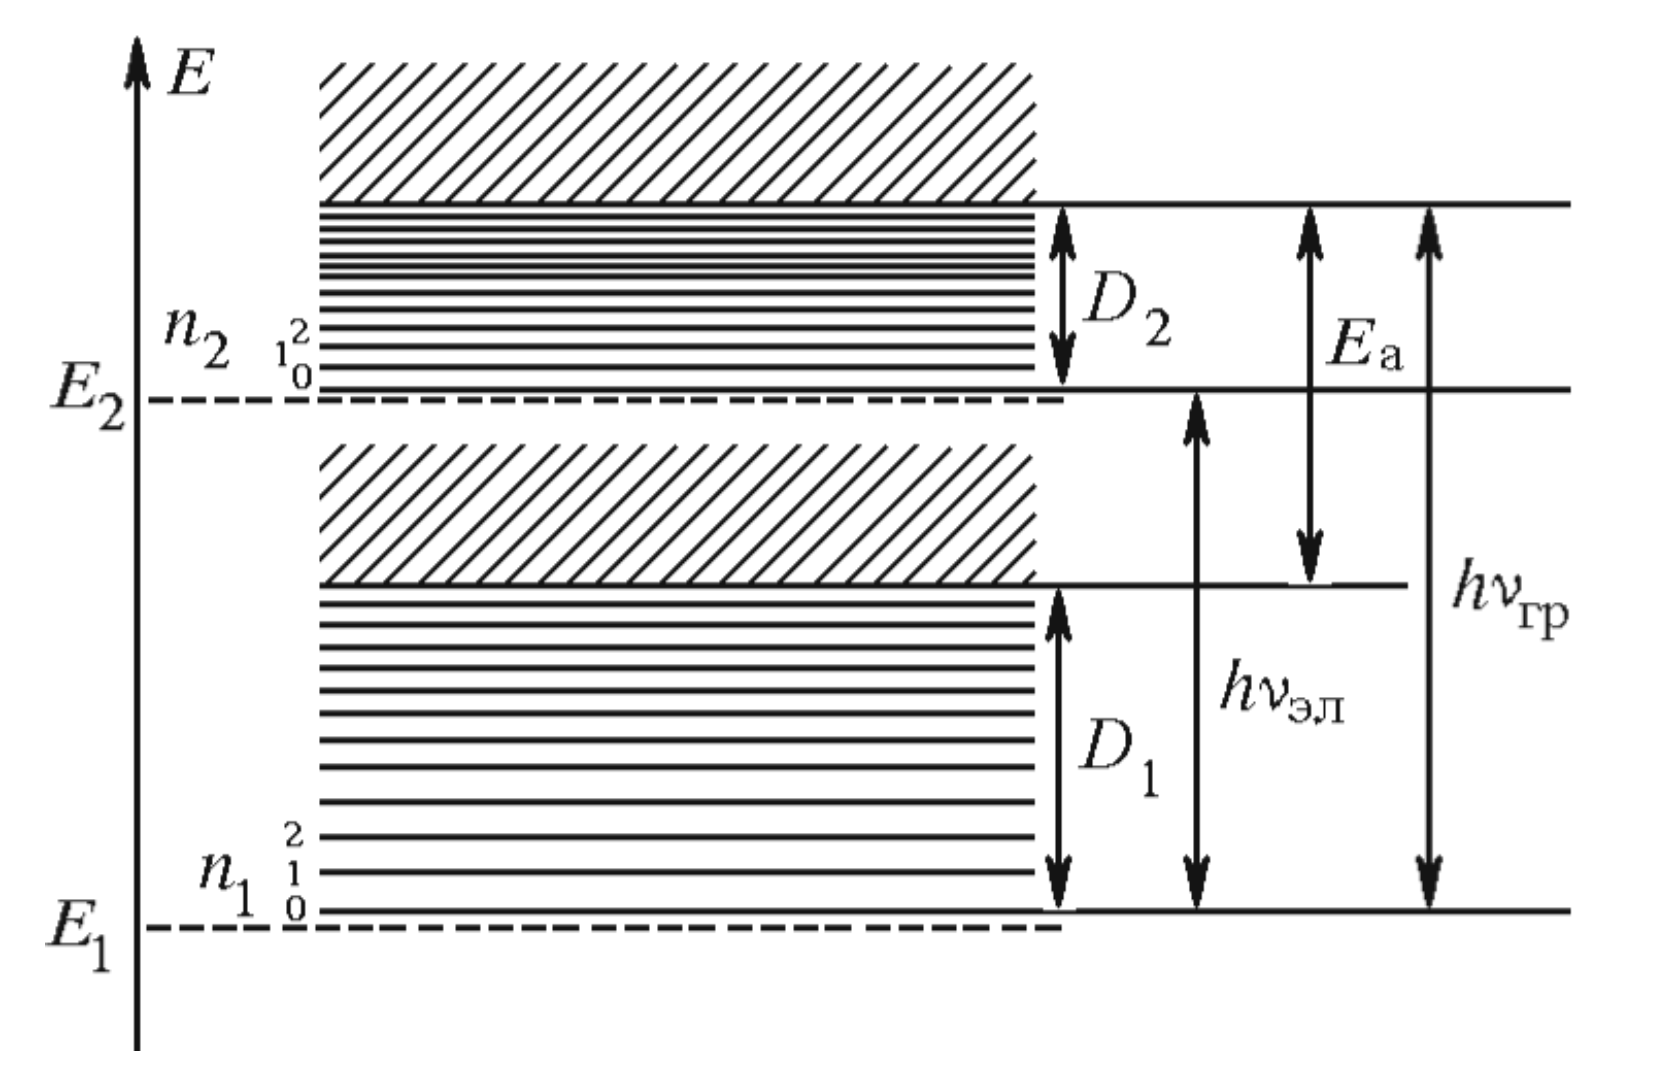
\includegraphics[width=0.5\textwidth]{molecular_energy.png}
\caption{Электронные и электронно-колебательные энергетические уровни двух-атомной молекулы}
\label{fig:molecule_en}
\end{figure}

\paragraph{} Оптические переходы (переходы, связанные с излучением фотонов в видимом диапазоне длин волн, т. е. фотонов с энергией порядка двух электрон-вольт) соответствуют переходам между различными электронными состояниями молекулы. При этом обычно происходят также изменения её вращательного и колебательного состояний. На рис. \ref{fig:molecule_en} показаны энергетические уровни двухатомной молекулы: электронные энергетические уровни обозначены пунктирными линиями, а электронно-колебательные сплошными линями. При больших колебательных энергиях электронно-колебательные уровни начинают сближаться. При слишком большой энергии колебания происходит диссоциация молекулы.

Энергетическое положение линий поглощения описывается выражением:
\begin{equation}
h \nu_{0, n_2} = E_2 - E_1 + h \nu_2 \left( n_2 + \frac{1}{2} \right) - \frac{h\nu_1}{2}
\label{e:molecule}
\end{equation}

\medskip\hrule\medskip

\section{Экспериментальная часть}

\subsection{Калибровка спектрометра}

\paragraph{} Приготовим спектрометр к работе. Добьёмся попадания сфокусированного света от неоновой лампы на входную щель спектрометра. Подберём размер щели таким образом, чтобы спектральные лини были отчётливо видны. Запишем показания барабана $\theta$ для различных спектральных линий. Проделаем то же самое для ртутной лампы. Данные записаны в таблице \ref{tab:calibration}. По полученным данным построим калибровочный график (рис. \ref{fig:calibration}). Калибровочную кривую найдём методом наименьших квадратов для многочлена четвёртой степени (даёт наилучшие результаты в данной задаче). Полученное значение:
\begin{equation}
f_\text{калиб}(\theta) = 1.036 \cdot 10^{-10} \theta^4 - 3.938 \cdot 10^{-7} \theta^3 + 0.0007589 \theta ^ 2 - 0.008151 \theta + 3986
\label{e:calibration}
\end{equation}
\noindent Точность определения показаний спектрометра $\Delta \theta \approx \pm 5$.  Точность определения длины волны:
\begin{equation}
\Delta \lambda = f'_\text{калиб}(\theta) \cdot \Delta \theta \approx (4.142 \cdot 10^{-10} \theta^3 - 1.181 \cdot 10^{-6} \theta^2 + 0.001518 \theta - 0.008151)\Delta \theta
\label{e:error}
\end{equation}

\begin{table}[]
\centering
\begin{tabular}{|c|c|c|c|c|c|c|c|c|}
\hline
Линия        & Ne, 1   & Ne, 2   & Ne, 3   & Ne, 4   & Ne, 5   & Ne, 6   & Ne, 7   & Ne, 8   \\ \hline
$\theta$     & 2638    & 2600    & 2542    & 2536    & 2500    & 2476    & 2466    & 2428    \\ \hline
$\lambda$, Å & 7032.41 & 6929.47 & 6717.04 & 6678.28 & 6598.96 & 6532.88 & 6506.53 & 6402.24 \\ \hline
Линия        & Ne, 9   & Ne, 10  & Ne, 11  & Ne, 12  & Ne, 13  & Ne, 14  & Ne, 15  & Ne, 16  \\ \hline
$\theta$     & Ne, 9   & Ne, 10  & Ne, 11  & Ne, 12  & Ne, 13  & Ne, 14  & Ne, 15  & Ne, 16  \\ \hline
$\lambda$, Å & 6382.99 & 6334.42 & 6304.79 & 6266.49 & 6217.26 & 6163.59 & 6143.06 & 6096.14 \\ \hline
Линия        & Ne, 17  & Ne, 18  & Ne, 19  & Ne, 20  & Ne, 21  & Ne, 22  & Ne, 23  & --      \\ \hline
$\theta$     & 2296    & 2278    & 2250    & 2234    & 2206    & 2186    & 1938    & --      \\ \hline
$\lambda$, Å & 6074.34 & 6030    & 5975.53 & 5944.83 & 5881.89 & 5852.49 & 5400.56 & --      \\ \hline
Линия        & Hg, 1   & Hg, 2   & Hg, 3   & Hg, 4   & Hg, 5   & Hg, 6   & --      & --      \\ \hline
$\theta$     & 2156    & 2142    & 1960    & 1542    & 874     & 314     & --      & --      \\ \hline
$\lambda$, Å & 5791    & 5770    & 5461    & 4916    & 4358    & 4047    & --      & --      \\ \hline
\end{tabular}
\caption{Калибровочные данные}
\label{tab:calibration}
\end{table}

\begin{figure}
\centering
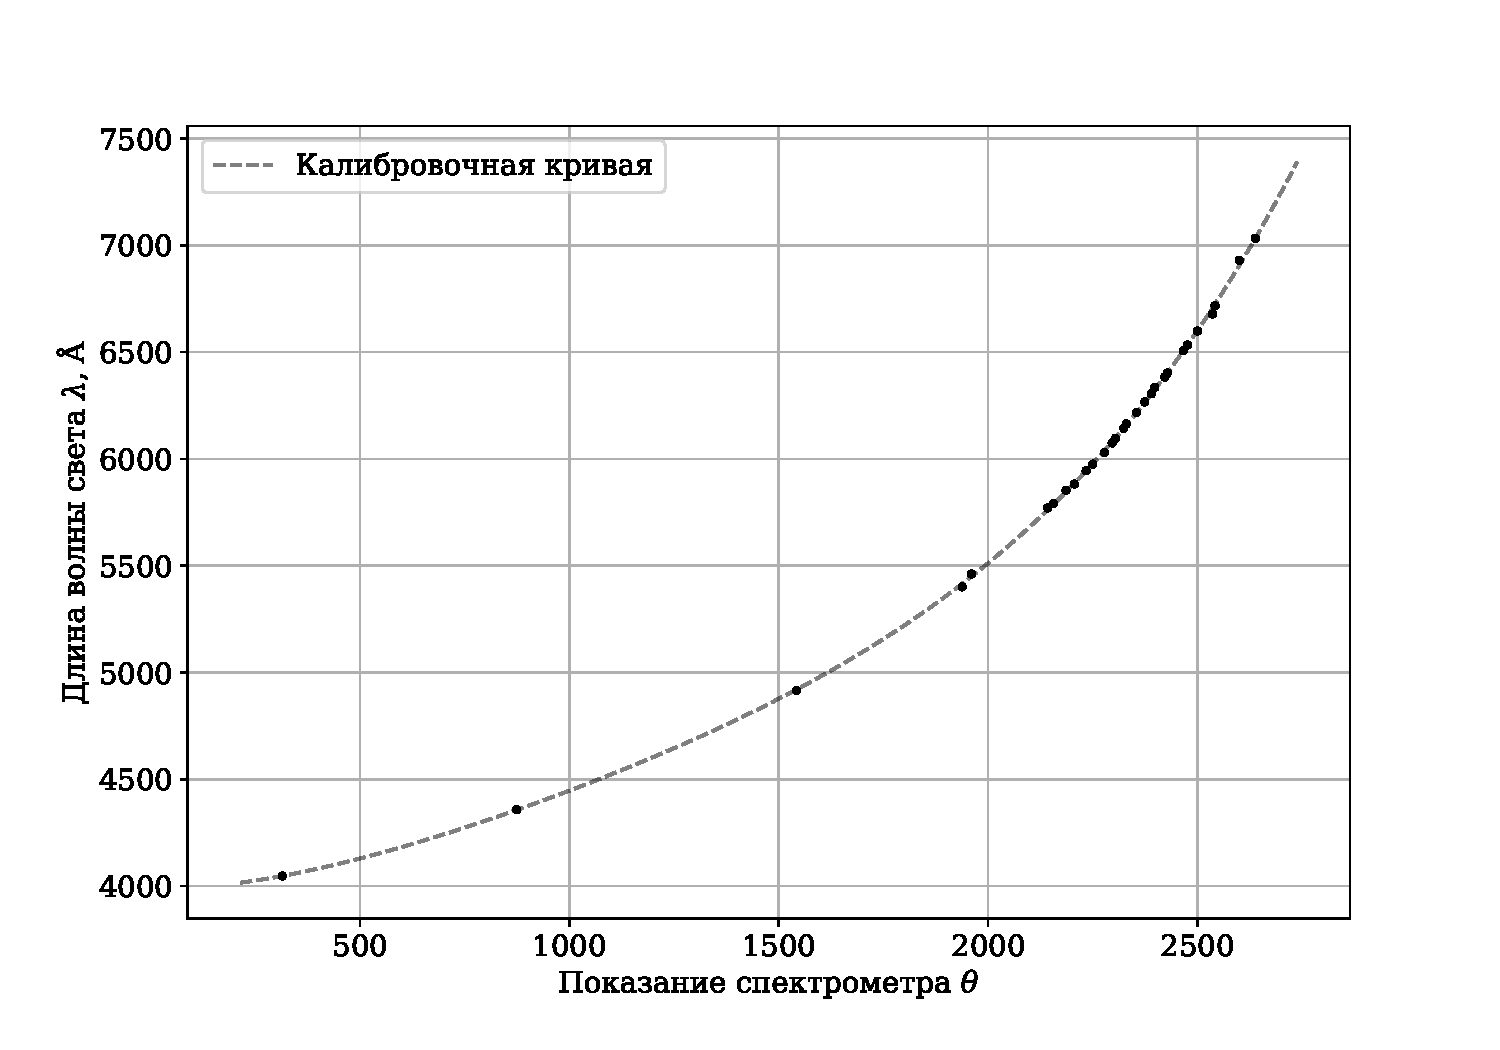
\includegraphics[width=\textwidth]{calibration.pdf}
\caption{Измеренные значения и калибровочный график}
\label{fig:calibration}
\end{figure}

\subsection{Спектр Водорода}

\paragraph{} Заменим ртутную лампу на водородную лампу. Получим в спектрометре изображение спектральных линий водорода. Измерим показание спектрометра для каждой линии, затем по калибровочному графику найдём длины волн спектров. Определим ошибки по формуле \eqref{e:error}. Данные запишем в табл. \ref{tab:h_spectrum}.

\begin{table}[]
\centering
\begin{tabular}{|l|c|c|c|c|}
\hline
Линия               & H$_\alpha$ & H$_\beta$ & H$_\gamma$ & H$_\delta$ \\ \hline
$\theta$            & 2486       & 1490      & 846        & 428        \\ \hline
$\lambda$, Å        & 6560       & 4867      & 4337       & 4094       \\ \hline
$\Delta \lambda$, Å & 15         & 5         & 4          & 3          \\ \hline
\end{tabular}
\caption{Спектральные линии водорода}
\label{tab:h_spectrum}
\end{table}

\paragraph{} По измеренным данным построим график зависимости $1/\lambda(n)$, где $n=3$ соответствует линии H$_\alpha$, $n=4$ -- H$_\beta$, $n=5$ -- H$_\gamma$, $n=6$ -- H$_\delta$ (рис. \ref{fig:ridberg}). Видим, что отношение длин волн соответствует формуле \eqref{e:balmer}. Найдём значение постоянной Ридберга $R$ построением кривой по формуле  \eqref{e:balmer} численным методом наименьших квадратов. Получим значение с погрешностью метода $R = 10.978 \pm 0.007$ мкм$^{-1}$


\begin{figure}
\centering
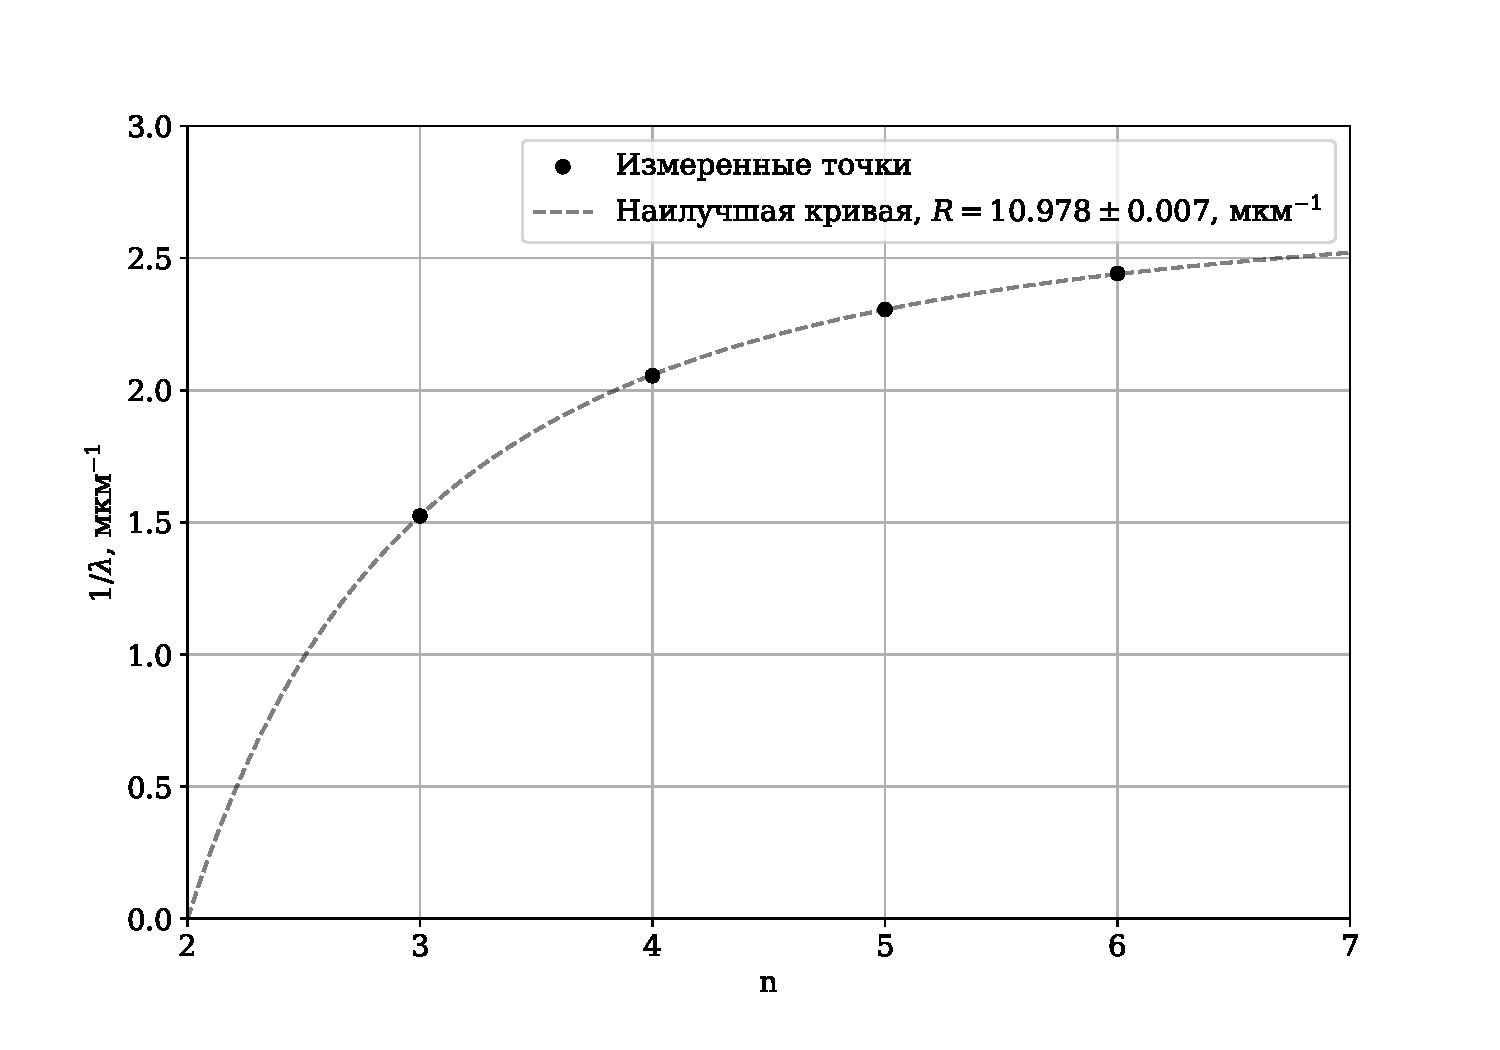
\includegraphics[width=\textwidth]{ridberg.pdf}
\caption{График зависимости $1/\lambda(n)$}
\label{fig:ridberg}
\end{figure}

\subsection{Спектр молекулы йода}

\paragraph{} Заменим водородную лампу на кювету с газом йода и осветим её сзади лампой накаливания. Получим на окуляре спектрометра серию тёмных полос поглощения. Найдём одну из самых длинноволновых хорошо видных линий поглощения ($n_{1, 0}$), линию ($n_{1, 5}$) -- шестой по счёту линии от выбранной, ($n_\text{гр}$) -- границу схождения спектра. Вычислим длины волн соответствующие этим линиям и энергии соответствующих квантов света, ошибки найдём по формуле \eqref{e:error}. Данные занесём в таблицу \ref{tab:i_spectrum}.

\begin{table}[]
\centering
\begin{tabular}{|c|c|c|c|c|c|}
\hline
Линия & $\theta$ & $\lambda$, Å & $\Delta \lambda$, Å & $\mathcal{E}_\varphi$, эВ & $\Delta \mathcal{E}_\varphi$, эВ \\ \hline
$n_{1, 0}$    & 2368 & 6249 & 13 & 1.984 & 0.004 \\ \hline
$n_{1, 5}$    & 2280 & 6043 & 11 & 2.052 & 0.004 \\ \hline
$n_\text{гр}$ & 1778 & 5192 & 7  & 2.388 & 0.003 \\ \hline
\end{tabular}
\caption{Спектральные линии йода}
\label{tab:i_spectrum}
\end{table}

\paragraph{} Вычислим энергию колебательного кванта возбуждённого состояния молекулы йода:
\[
\mathcal{E}_2 = \frac{\mathcal{E}_{1, 5} - \mathcal{E}_{1, 0}}{5} = 0.0136 \text{ эВ}, \; \Delta\mathcal{E}_2 = \frac{\sqrt{\Delta\mathcal{E}_{1, 5}^2 - \Delta\mathcal{E}_{1, 0}^2}}{5} \approx 0.001 \text{ эВ},
\]
\noindent получили $h \nu_2 = 0.014 \pm 0.001$ эВ.

\paragraph{} Пользуясь тем, что энергия колебательного кванта в основном состоянии $h \nu_1 = 0.027$ эВ, а энергия возбуждения атом $E_A = 0.94$ эВ, найдём энергию электронного перехода по формуле \eqref{e:molecule}:
\[
h \nu_\text{эл} = h \nu_{1, 0} - \frac{h \nu_2}{2} + \frac{3h \nu_1}{2} = 2.017 \pm 0.004 \text{ эВ}.
\]

Определим энергию диссоциации молекулы в основном $D_1$ и возбуждённом состоянии $D_2$:
\[
D_1 = h \nu_\text{гр} - E_A = 1.448 \pm 0.003 \text{ эВ}, \; D_2 = h \nu_\text{гр} - h \nu_\text{эл} = 0.371 \pm 0.005 \text{ эВ}.
\]

\medskip\hrule\medskip

\section{Выводы}

\begin{enumerate}
\item Получили калибровочный график для спектрометра. Оценили погрешность значений.
\item Измерили спектр водорода. По полученным данным проверили формулу Ридберга и получили значение постоянной Ридберга $R = 10.978 \pm 0.007$ мкм$^{-1}$, что соответствует табличному значению $10. 973731$ мкм$^{-1}$.
\item Нашли энергии: колебательного кванта возбуждённого состояния молекулы йода $h \nu_2 = 0.014 \pm 0.001$ эВ, электронного перехода $h \nu_\text{эл} = 2.017 \pm 0.004 \text{ эВ}$, диссоциации молекулы в основном состоянии $D_1 = 1.448 \pm 0.003 \text{ эВ}$, диссоциации молекулы в возбуждённом состоянии $D_2 =  0.371 \pm 0.005 \text{ эВ}$.
\end{enumerate}

\medskip\hrule\medskip

\end{document}
